%%%
%%% COMPATIBILITY NOTION
%%%
\section{Towards a Notion of Compatibility}
\label{chap:compatibility:informal}

\mnote{Modular relations induce monolithic ones}
We start with general considerations on \modellevelconsistencyrelations, be they specified explicitly or implied by sets of fine-grained consistency relations.
A set of binary \modellevelconsistencyrelations induces a monolithic, multiary relation, also called \emph{global relation}, as discussed in \autoref{chap:correctness:notions_correctness:relations}.
A monolithic relation $\consistencyrelation{CR}{}$ for metamodels $\metamodelsequence{M}{n}$ and pairwise consistency relations $\consistencyrelation{CR}{i,j}$ is defined by:
\begin{align*}
    \consistencyrelation{CR}{} = \setted{\tupled{\model{m}{1}, \dots, \model{m}{n}} \mid \bigwedge\limits_{1 \le i < j \le n} \tupled{\model{m}{i}, \model{m}{j}} \in \consistencyrelation{CR}{i,j}}
\end{align*}
As discussed before, the consistency relations are correct by definition and so is the induced global relation, even if it is empty.
It is, however, unclear whether the relations are reasonable in combination.
%However, just because the induced monolithic relation does, for example, only contain one consistent tuple of models, this may not imply that it is not as intended.

\begin{figure}
    \centering
    \newcommand{\mdistance}{2.5em}

\begin{tikzpicture}[
    model/.style={schematic model, minimum size=2em, inner sep=0.1em},
    correspondence/.style={consistency related element, -}
]

\pgfdeclarelayer{bg}
\pgfdeclarelayer{main}
\pgfsetlayers{bg,main}

\node[model] (m11) {$\model{m}{1}'$};
\node[model, below right=0.615*\mdistance and 1.143*\mdistance+0.7*\mdistance of m11.center, anchor=center] (m1) {$\model{m}{1}$};
\node[below=0.8*\mdistance of m11.center, anchor=center] (m1_label) {$\metamodelinstanceset{M}{1}$};

\node[model, right=8*\mdistance of m11.center, anchor=center] (m21) {$\model{m}{2}'$};
\node[model, below left=0.615*\mdistance and 1.143*\mdistance+0.7*\mdistance of m21.center, anchor=center] (m2) {$\model{m}{2}$};
\node[below=0.8*\mdistance of m21.center, anchor=center] (m2_label) {$\metamodelinstanceset{M}{2}$};

\node[model, below right=3.5*\mdistance and 4*\mdistance of m11.center, anchor=center] (m31) {$\model{m}{3}'$};
\node[model, above=\mdistance of m31.center, anchor=center] (m3) {$\model{m}{3}$};
\node[right=1.5em of m31.center, anchor=west] (m3_label) {$\metamodelinstanceset{M}{3}$};

\begin{pgfonlayer}{bg}
    \node[schematic metamodel, ellipse, fit=(m11)(m1)(m1_label.center)] {};
    \node[schematic metamodel, ellipse, fit=(m21)(m2)(m2_label.center)] {};
    \node[schematic metamodel, ellipse, fit=(m31)(m3)(m3_label.center)] {};
\end{pgfonlayer}

\draw[correspondence] (m11) to [bend left=3] (m2);
\draw[correspondence] (m1) to [bend left=3] (m21);
\draw[correspondence] (m11) -- (m31);
\draw[correspondence] (m1) -- (m3);
\draw[correspondence] (m2) -- (m3);
\draw[correspondence] (m21) -- (m31);

\node[consistency related element, yshift=2.5em] at ($(m11)!0.5!(m21)$) {$\consistencyrelation{CR}{1,2} = \setted{\tupled{\model{m}{1},\model{m}{2}'}, \tupled{\model{m}{1}',\model{m}{2}}}$};
\node[consistency related element, xshift=1em, anchor=north east, align=center] at ($(m11)!0.5!(m31)$) {$\consistencyrelation{CR}{1,3} =$ \\ $\setted{\tupled{\model{m}{1},\model{m}{3}}, \tupled{\model{m}{1}',\model{m}{3}'}}$};
\node[consistency related element, xshift=-1em, anchor=north west, align=center] at ($(m21)!0.5!(m31)$) {$\consistencyrelation{CR}{2,3} =$ \\ $\setted{\tupled{\model{m}{2},\model{m}{3}}, \tupled{\model{m}{2}',\model{m}{3}'}}$};

\end{tikzpicture}
    %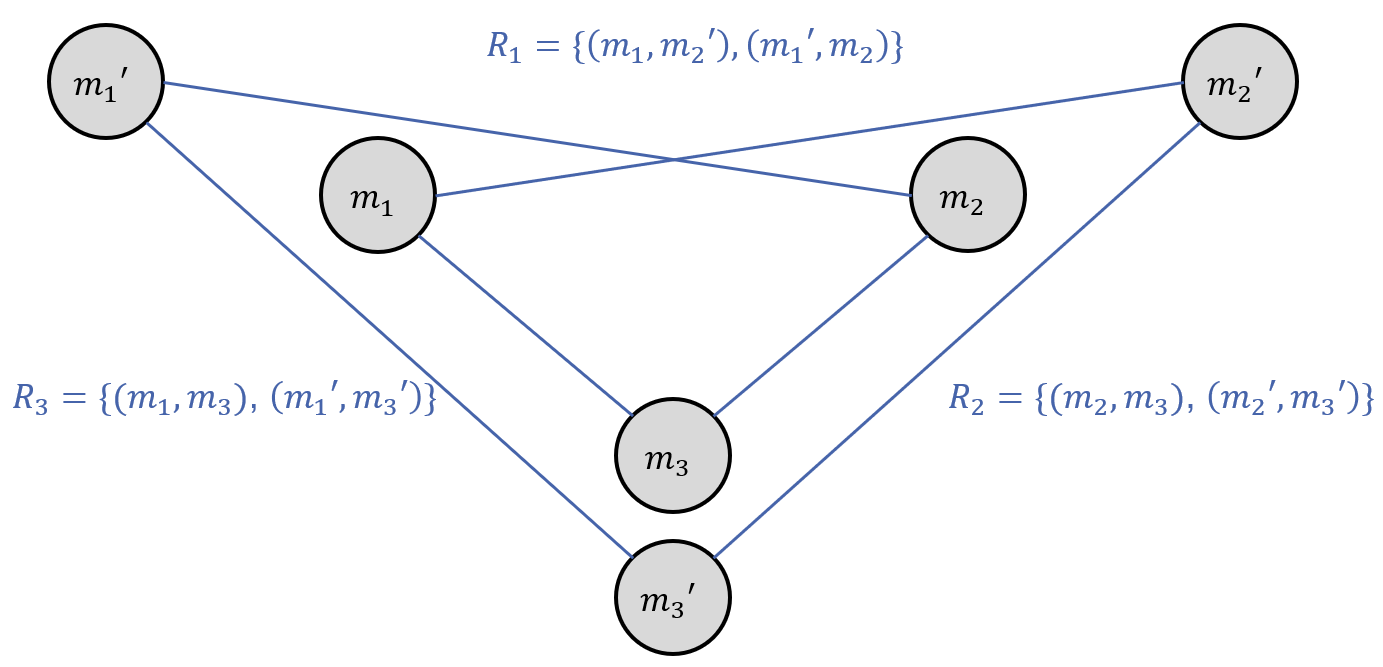
\includegraphics[width=\textwidth]{figures/correctness/compatibility/empty_global_relation.png}
    \caption[Consistency relations that imply an empty global relation]{Example for consistency relations that imply an empty global relation.}
    \label{fig:compatibility:empty_global_relation}
\end{figure}

\mnote{Empty induced global relations}
In fact, if the relations induce an empty global relation, these relations do actually not properly fit to each other, because no single tuple of models would be considered consistent, thus no system could be consistently described.
One may thus consider such relations incompatible.
\autoref{fig:compatibility:empty_global_relation} shows an extended version of the example already given in \autoref{chap:correctness:notions_correctness:relations}, which induces an empty global relation.
This is an abstraction of the concrete examples that we have already discussed for our our running example, in which modified consistency relations lead to an empty set of consistent model tuples due to conflicting conversions and concatenations of names between persons, residents and employees.

\mnote{Goal of identifying incompatible relations}
There may, however, be more cases than empty induced global relations that we want to exclude by considering the relations incompatible.
In general, the goal of finding incompatibilities and excluding them is twofold:
First, we want to identify that different developers of modular relations have an incompatible notion of consistency, such that the results of preserving consistency would never be as expected.
This is what we have seen in the examples with the name relations.
We want to exclude these cases, because developers will not want to combine transformations based on relations that are contradicting.
Second, incompatibilities may lead to transformations not being able to find consistent models, so the orchestration would not be able to execute transformations in an order that achieves a consistent state.
If we, for example, encoded the relations from the running example with the inverse concatenation of $\mathvariable{firstname}$ and $\mathvariable{lastname}$ ($\consistencyrelation{CR}{PR}'$) into transformations, each cycle in which the transformations are executed would produce one new person, employee and resident, or change each of the existing ones, such that $\mathvariable{firstname}$ and $\mathvariable{lastname}$ are swapped and a comma is appended to $\mathvariable{lastname}$.
In consequence, transformations would not be able to find a consistent state and, if not stopped preemptively, be executed endlessly.
Thus, we also want to exclude such cases, because they can prevent the execution of transformations in a transformation network from terminating.

%\begin{itemize}
    %\item We discussed that we are not interested in correctness of modular relations w.r.t. one monolithic relations, as that relations is usually unknown and thus correctness cannot be checked (cf ~\autoref{chap:correctness:notions:dimensions})
    %\item This would mean that modular relations are correct by construction
    %\item Although relations are, theoretically, correct by construction, we have seen that there are relations, for which we may say that they do not properly work together, i.e., they are \emph{incompatible}, as discussed in \autoref{chap:correctness:notions:relations}
    %\item There, we had three binary relations, which, taken together, do not impose an overall relation containing any consistent set of models, see \autoref{fig:compatibility:empty_global_relation}
    %\item We have already given a more concrete example for that case from our running example before.
    %\item It is obvious that we may not want to have an induced global relation that is empty, however, there may be more cases that we want to exclude.
    %%\item Exclude somehow defined \emph{incompatibilities} may be wanted for two reasons: First, we may want to identify that different developers of modular relations have an incompatible notion of consistency, such that the result would never be as expected (this is what we have seen for the names). Second, incompatibilities may lead to transformations not being able to find a consistent solution, so the orchestration would not be able to execute transformations to achieve a consistent state. To show that, we extend the relations example to a transformation example, showing that no consistent state can be reached, i.e., for an added person no consistent employees etc. can be found
%\end{itemize}


%%
%% OBSOLETE RELATIONS
%%
\subsection{Necessity of Obsolete Relation Elements}

\begin{figure}
    \centering
    \newcommand{\mdistance}{2.5em}

\begin{tikzpicture}[
    model/.style={schematic model, minimum size=2em, inner sep=0.1em}
]

\pgfdeclarelayer{bg}
\pgfsetlayers{bg,main}

\node[model] (m11) {$\model{m}{1}'$};
\node[model, below right=0.615*\mdistance and 1.143*\mdistance+0.7*\mdistance of m11.center, anchor=center] (m1) {$\model{m}{1}$};
\node[below=0.8*\mdistance of m11.center, anchor=center] (m1_label) {$\metamodelinstanceset{M}{1}$};

\node[model, right=8*\mdistance of m11.center, anchor=center] (m21) {$\model{m}{2}'$};
\node[model, below left=0.615*\mdistance and 1.143*\mdistance+0.7*\mdistance of m21.center, anchor=center] (m2) {$\model{m}{2}$};
\node[below=0.8*\mdistance of m21.center, anchor=center] (m2_label) {$\metamodelinstanceset{M}{2}$};

\node[model, below right=3.5*\mdistance and 4*\mdistance of m11.center, anchor=center] (m31) {$\model{m}{3}'$};
\node[model, above=\mdistance of m31.center, anchor=center] (m3) {$\model{m}{3}$};
\node[right=1.5em of m31.center, anchor=west] (m3_label) {$\metamodelinstanceset{M}{3}$};

\begin{pgfonlayer}{bg}
    \node[schematic metamodel, ellipse, fit=(m11)(m1)(m1_label.center)] {};
    \node[schematic metamodel, ellipse, fit=(m21)(m2)(m2_label.center)] {};
    \node[schematic metamodel, ellipse, fit=(m31)(m3)(m3_label.center)] {};
\end{pgfonlayer}

\draw[correspondence] (m11) to [bend left=3] (m2);
\draw[correspondence] (m11) -- (m21);
\draw[correspondence] (m1) to [bend left=3] (m21);
\draw[correspondence] (m1) -- (m2);
\draw[correspondence] (m11) -- (m31);
\draw[correspondence] (m1) -- (m3);
\draw[correspondence] (m2) -- (m3);
\draw[correspondence] (m21) -- (m31);

\node[consistency related element, yshift=3em] at ($(m11)!0.5!(m21)$) {$\consistencyrelation{CR}{1,2} = \setted{\tupled{\model{m}{1},\model{m}{2}}, \tupled{\model{m}{1},\model{m}{2}'}, \tupled{\model{m}{1}',\model{m}{2}}, \tupled{\model{m}{1}',\model{m}{2}'}}$};
\node[consistency related element, xshift=1em, anchor=north east, align=center] at ($(m11)!0.5!(m31)$) {$\consistencyrelation{CR}{1,3} =$ \\ $\setted{\tupled{\model{m}{1},\model{m}{3}}, \tupled{\model{m}{1}',\model{m}{3}'}}$};
\node[consistency related element, xshift=-1em, anchor=north west, align=center] at ($(m21)!0.5!(m31)$) {$\consistencyrelation{CR}{2,3} =$ \\ $\setted{\tupled{\model{m}{2},\model{m}{3}}, \tupled{\model{m}{2}',\model{m}{3}'}}$};

\end{tikzpicture}
    %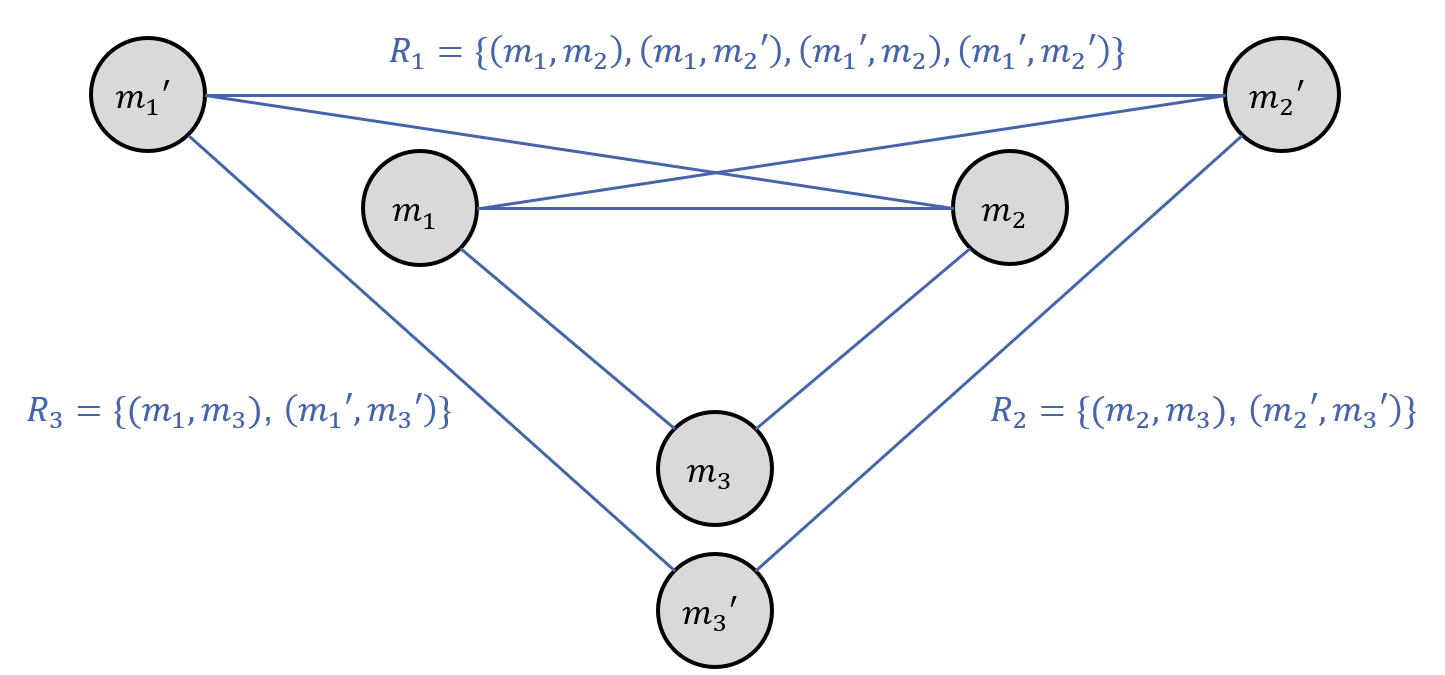
\includegraphics[width=\textwidth]{figures/correctness/compatibility/obsolete_relations.png}
    \caption[Example for obsolete elements in consistency relations]{Example for obsolete model pairs in consistency relation $\consistencyrelation{CR}{1,2}$, which can never occur in a globally consistent tuple of models.}
    \label{fig:compatibility:obsolete_relations}
\end{figure}

\mnote{Obsolete model pairs}
A first intuitive option to define incompatibility is the presence of model pairs in the consistency relations, for which no globally consistent model tuple containing them can be found.
This canonically covers the case in which the modular relations induce an empty global relation, because for none of the model pairs in each relation a globally consistent model tuple containing them can be found.
An example for that case is depicted in \autoref{fig:compatibility:obsolete_relations}, in which the relation $\consistencyrelation{CR}{1,2}$ contains the pairs $\tupled{\model{m}{1}, \model{m}{2}'}$ and $\tupled{\model{m}{1}', \model{m}{2}}$, for which neither $\model{m}{3}$ nor $\model{m}{3}'$ is consistent to both other consistency relations, as the induced global relation is $\consistencyrelation{CR}{} = \setted{\tupled{\model{m}{1},\model{m}{2},\model{m}{3}},\tupled{\model{m}{1}',\model{m}{2}',\model{m}{3}'}}$.
Thus, these model pairs may be denoted \emph{obsolete} as they cannot occur in any globally consistent model tuple.

\mnote{Forbidding obsolete model pairs}
While this point of view may be reasonable when considering only the consistency relations, as we are finally just interested in results that are globally consistent, it induces problems to the process of achieving such a result by means of the execution of transformations or, more precisely, their consistency preservation rules.
In fact, transformation networks need to allow intermediate states of models that are only locally consistent, although they can never occur in a globally consistent state.
This is necessary, because otherwise each transformation would have to consider which model pairs are not only locally consistent but can be globally consistent as well.
We, however, excluded such an alignment of the transformations by assumption of independent development and modular reuse and instead let the orchestration of transformations negotiate a consistent result.

\begin{figure}
    \centering
    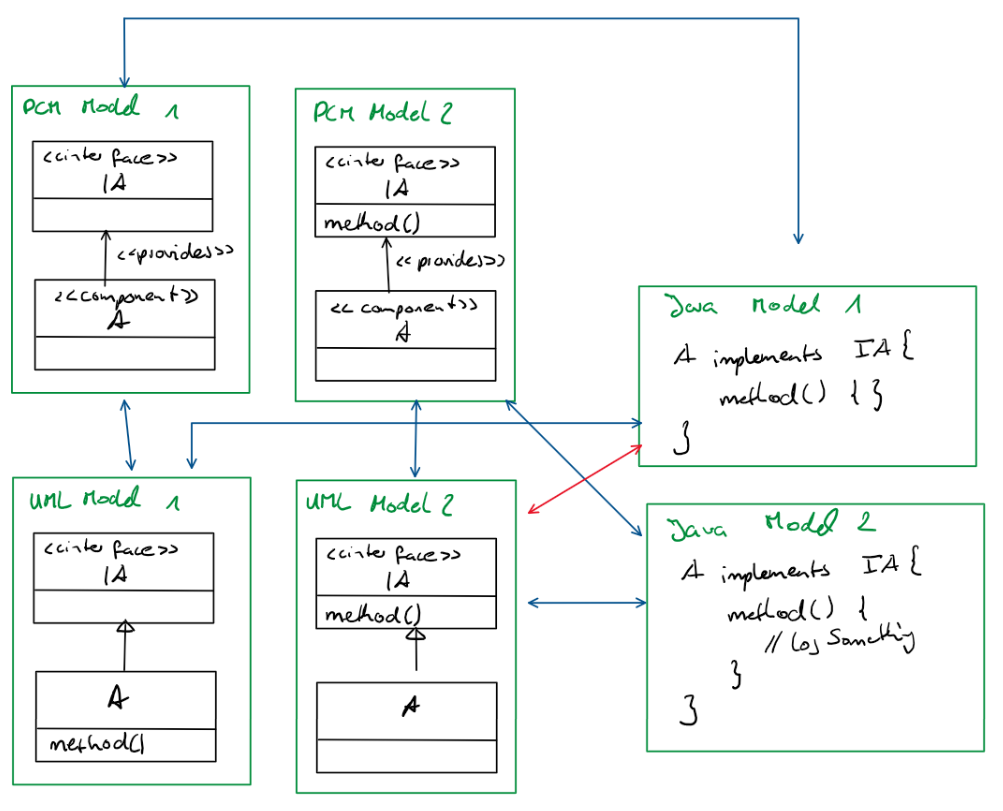
\includegraphics[width=\textwidth]{figures/correctness/compatibility/obsolete_relations_scenario.png}
    \caption[Concrete scenario with obsolete relation elements]{Example for an obsolete model pair in consistency relations between \gls{PCM}, UML and Java: The empty Java method realization is locally consistent to the UML class model that defines the method in the class interface, but cannot be globally consistent because it realizes a \gls{PCM} component, for which the consistency relation requires at least a default implementation.}
    \label{fig:compatibility:obsolete_relations_scenario}
\end{figure}

\mnote{Example for obsolete relation necessity}
Consider the following example, which is also exemplarily depicted in \autoref{fig:compatibility:obsolete_relations_scenario}.
A UML class model and Java code are considered consistent when the same classes and interfaces with the same methods (in Java potentially with an empty body) are contained.
In fact, for each UML model a usually infinite number of consistent Java models exists, containing arbitrary implementations of the methods.
In addition, \gls{PCM} models and UML class models are consistent when components are realized as classes implementing the provided interfaces of the components and thus their methods.
Analogously, each component is represented by a Java class implementing the provided interface.
The consistency relation between \gls{PCM} and Java may, however, require that a method within a class that realizes a method of a provided interface of a component has at least some default implementation, be it logging or something more component-specific.
%The transformation between \gls{UML} and Java may initialize a method added to a class with an empty body or dummy return statement.
%The transformation between \gls{PCM} and Java may, however, initializes a method within a class that realizes a component with a default implementation, be it logging or something more component-specific.
If we considered model pairs that can never occur in globally consistent model tuples as incompatible and thus forbid them, a UML model could not be considered consistent to a Java model if any method in a class that realizes a component and that is defined by one of its interfaces is realized by a Java method with an empty body.
The transformation between UML and Java would thus not be allowed to create an empty Java method upon creation of a UML method.
This would, however, enforce the relation between UML and Java to encode information about components, which both breaks our assumption of independent development, as the developer of the transformation between UML and Java would need to know about components, and of modular reuse, because the transformation is then tied to the scenario in which \gls{PCM} is used as well.

\mnote{No proper notion of incompatibility}
In consequence of the given scenario and the according insight that transformations may need to produce transient states that are only locally consistent to ensure independence of the transformations and their reusability in different contexts, such obsolete consistency relations do not induce a proper notion of incompatibility.

%First option: Remove "obsolete" relation elements

% \begin{itemize}
%     \item A first option might be to say that there should not be model pairs in the relations for which no globally consistent set of models can be found (give an abstract example for that)
%     \item However, in consequence a transformation could not produce such models, which might be necessary as transient (intermediate) states: E.g., a UML and Java code model are consistent when the same classes and interface with the same (in Java potentially empty) methods are present. In fact, a UML model is consistent with all (usually infinite) Java models with the same classes and methods, but with arbitrary method implementation. PCM and UML are consistent when components are realized as classes implementing the provided interfaces and thus their methods. Analogously, each component is represented by a Java class implementing the provided interfaces, but having an implementation that has some default functionality (be it logging or something more component-specific). 
%     Forbidding relations elements that can never be globally consistent would forbid that the relation between UML and Java allows Java models with empty method implementations for UML classes representing components. This would, however, require the relation/transformation between UML and Java know about components, which should not be the case due to modularity and independent development. Additionally, even in the concrete setup in which PCM is used, if a method is added to an interface of a class in UML which is a provided interface of its component in UML, the transformations may first create the Java method with an empty body, then propagate the method to the PCM interface and then propagate the default implementation of that method from PCM to Java. In this case, the transient state with the empty method body in Java is passed. Forbidding that would require an appropriate orchestration, i.e., first propagating the information across PCM, which could be defined for this specific case but not automatically decided in general, or the UML-Java transformation would have to consider that the Java implementation may not be empty, which, as discussed, contradicts modularity.
%     \item In general, this case is reflected in \autoref{fig:compatibility:obsolete_relations}, which shows two pairs in $R_1$, which can never occur in a globally consistent model, because the implied global relation is .... and does not contain those model pairs
% \end{itemize}


%%
%% UNWANTED BEHAVIOR
%%
\subsection{Prevention from Finding Consistent Solutions}
\label{chap:compatibility:informal:prevention}

% Second attempt: Derive incompatibility notion from unwanted behavior
\begin{figure}
    \centering
    \newcommand{\mdistance}{2.5em}

\begin{tikzpicture}[
    model/.style={schematic model, minimum size=2em, inner sep=0.1em},
    correspondence/.style={consistency related element, -}
]

\pgfdeclarelayer{bg}
\pgfsetlayers{bg,main}

\node[model] (m11) {$\model{m}{1}'$};
\node[model, below right=0.615*\mdistance and 1.143*\mdistance+0.7*\mdistance of m11.center, anchor=center] (m1) {$\model{m}{1}$};
\node[model, above left=0.615*\mdistance and 1.143*\mdistance+0.7*\mdistance of m11.center, anchor=center] (m12) {$\model{m}{1}''$};
\node[below=1.2*\mdistance of m12.center, anchor=center] (m1_label) {$\metamodelinstanceset{M}{1}$};

\node[model, right=7.5*\mdistance of m11.center, anchor=center] (m21) {$\model{m}{2}'$};
\node[model, below left=0.615*\mdistance and 1.143*\mdistance+0.7*\mdistance of m21.center, anchor=center] (m2) {$\model{m}{2}$};
\node[below=0.8*\mdistance of m21.center, anchor=center] (m2_label) {$\metamodelinstanceset{M}{2}$};

\node[model, below right=3.5*\mdistance and 3.75*\mdistance of m11.center, anchor=center] (m31) {$\model{m}{3}'$};
\node[model, above=\mdistance of m31.center, anchor=center] (m3) {$\model{m}{3}$};
\node[right=1.5em of m31.center, anchor=west] (m3_label) {$\metamodelinstanceset{M}{3}$};

\begin{pgfonlayer}{bg}
    \node[schematic metamodel, ellipse, fit=(m11)(m1)(m12)(m1_label.center)] {};
    \node[schematic metamodel, ellipse, fit=(m21)(m2)(m2_label.center)] {};
    \node[schematic metamodel, ellipse, fit=(m31)(m3)(m3_label.center)] {};
\end{pgfonlayer}

\draw[correspondence] (m12) to [bend left=3] (m21);
\draw[correspondence] (m11) to [bend left=5] (m2);
\draw[correspondence] (m1) to [bend left=5] (m21);
\draw[correspondence] (m1) -- (m2);
\draw[correspondence] (m11) -- (m31);
\draw[correspondence] (m12) -- (m31);
\draw[correspondence] (m1) -- (m3);
\draw[correspondence] (m2) -- (m3);
\draw[correspondence] (m21) -- (m31);

\node[consistency related element, yshift=4em] at ($(m12)!0.5!(m21)$) {$\consistencyrelation{CR}{1,2} = \setted{\tupled{\model{m}{1},\model{m}{2}}, \tupled{\model{m}{1},\model{m}{2}'}, \tupled{\model{m}{1}',\model{m}{2}}, \tupled{\model{m}{1}'',\model{m}{2}'}}$};
\node[consistency related element, xshift=1em, anchor=north east, align=center] at ($(m12)!0.65!(m31)$) {$\consistencyrelation{CR}{1,3} =$ \\ $\setted{\tupled{\model{m}{1},\model{m}{3}}, \tupled{\model{m}{1}',\model{m}{3}'}, \tupled{\model{m}{1}'',\model{m}{3}'}}$};
\node[consistency related element, xshift=-1em, anchor=north west, align=center] at ($(m21)!0.47!(m31)$) {$\consistencyrelation{CR}{2,3} =$ \\ $\setted{\tupled{\model{m}{2},\model{m}{3}}, \tupled{\model{m}{2}',\model{m}{3}'}}$};

\node[below left=4.3*\mdistance and 1.1*\mdistance of m12.west, anchor=north west, align=left, inner sep=0em] {
    $\begin{aligned}
        & \text{Input: } 
            \tupled{\model{m}{1},\model{m}{2},\model{m}{3}} \rightarrow \tupled{\model{m}{1},\model{m}{2}',\model{m}{3}}\\
        & \text{Execution: }
            \rightarrow \model{m}{3}' \rightarrow \model{m}{1}' \rightarrow \model{m}{2} \rightarrow \model{m}{3} \rightarrow \model{m}{1} \\
        & \text{Output: }
            \tupled{\model{m}{1},\model{m}{2},\model{m}{3}}
    \end{aligned}$
};

\end{tikzpicture}
    %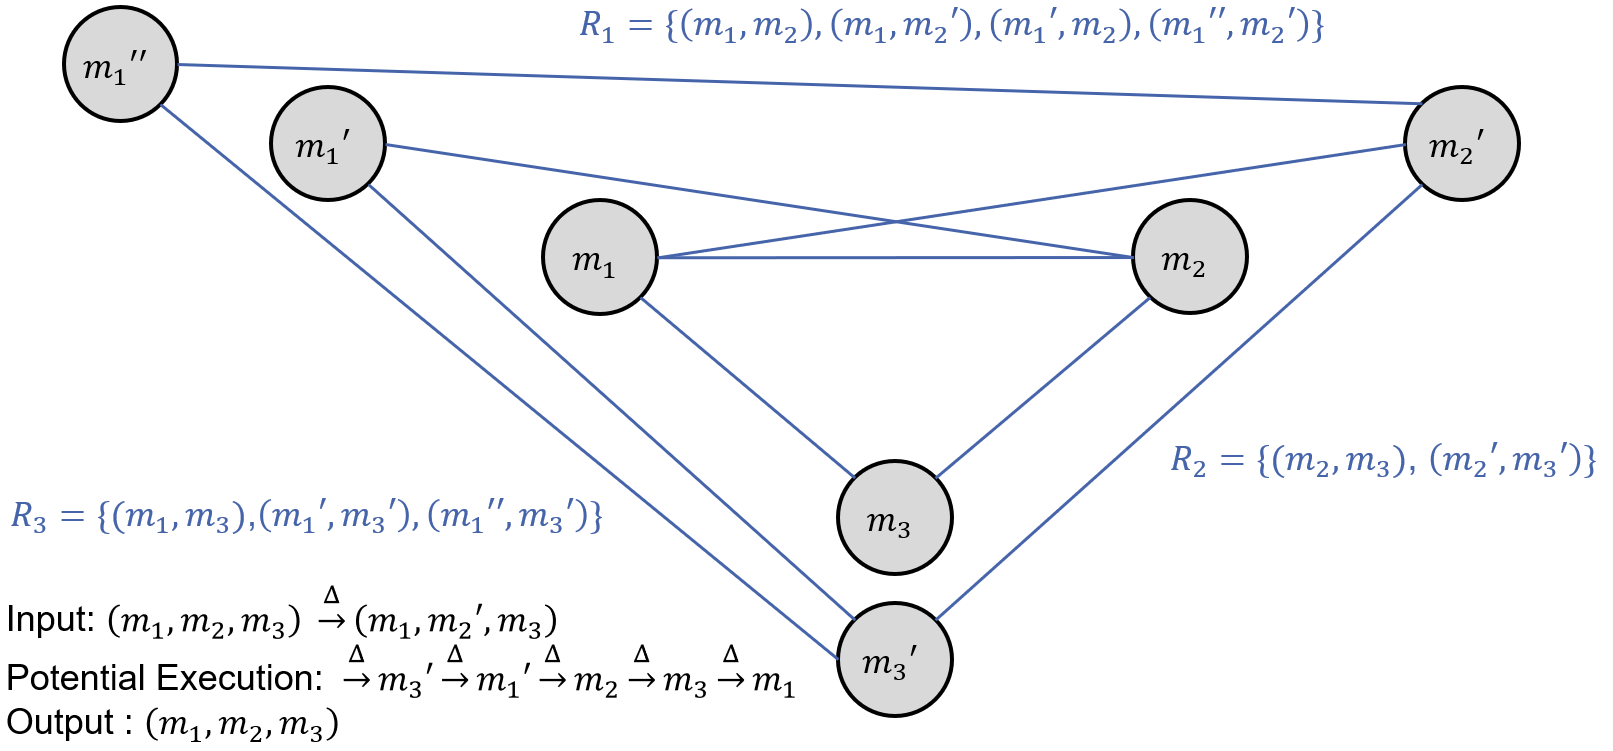
\includegraphics[width=\textwidth]{figures/correctness/compatibility/unwanted_behavior.png}
    \caption[Example for the unwanted rejection of a user change]{Example for the rejection of a user change because of consistency relations containing model pairs that are never globally consistent.}
    \label{fig:compatibility:unwanted_behavior}
\end{figure}

\mnote{Reverting user changes}
To identify a proper notion of incompatibility, we consider an exemplary transformation scenario from which we can derive such a notion.
In the example depicted in \autoref{fig:compatibility:unwanted_behavior}, we start with the models $\model{m}{1}$, $\model{m}{2}$ and $\model{m}{3}$, which are consistent to all three defined consistency relations.
If a user performs a change of $\model{m}{2}$ to $\model{m}{2}'$, one possible execution of transformation can look as follows:
The transformation for $\consistencyrelation{CR}{2,3}$ changes $\model{m}{3}$ to $\model{m}{3}'$, the one for $\consistencyrelation{CR}{1,3}$ changes $\model{m}{1}$ to $\model{m}{1}'$ and then the one for $\consistencyrelation{CR}{1,2}$ changes $\model{m}{2}'$ back to $\model{m}{2}$, as that is the only model consistent to $\model{m}{1}'$.
Now the transformation for $\consistencyrelation{CR}{2,3}$ changes $\model{m}{3}'$ back to $\model{m}{3}$ and finally the one for $\consistencyrelation{CR}{1,3}$ restores $\model{m}{1}$.
As a result, the determined execution order results in returning the initial models before the user change, which are actually consistent but reject the user change.

\mnote{Bad local selections} %Unnecessarily bad local selections can prevent network from finding proper solution
Apart from the three given models, only $\model{m}{1}''$, $\model{m}{2}'$ and $\model{m}{3}'$ are consistent.
Upon the user change of $\model{m}{2}$ to $\model{m}{2}'$, we would actually expect the transformations to find the latter triple of models as a consistent result, as otherwise, like in the above example, the original models are returned, which actually rejects the user change.
The problem results from the model $\model{m}{1}'$ being present in the consistency relations, but not being consistent in any globally consistent model tuple.
For each of the transformations the local selection of $\model{m}{1}'$ is fine, as there are models to which it is locally consistent according to each consistency relation on its own.

\mnote{Difference to obsolete elements} %Scenario is different from obsolete relation elements}
Note that this scenario is different from the case discussed for obsolete relation elements.
In the scenarios discussed for obsolete relation elements, each model in such an obsolete pair occurs in a globally consistent model tuple, but not both models in that pair together do.
For example, the Java class with an empty method body actually occurs in a globally consistent model tuple, but not together with the UML class model in which the method is defined in the class interface, although they are locally consistent.

\mnote{Relation to user changes} %Models that do not occur in any globally consistent model tuple are problematic
We have seen that it is problematic when consistency relations define consistency of models that do not occur in any globally consistent model tuple.
This can easily lead to transformations that do not find expected solutions and unnecessarily reject user changes.
We did not define a requirement that user changes may not be reverted on purpose, as that behavior may also be expected to express that certain changes are not allowed to be made.
However, if there was a reasonable sequence of transformations that returns a consistent tuple of models reflecting the user changes, it should be preferred over one that reverts the user change.

% \begin{itemize}
%     \item Considering the example in \autoref{fig:compatibility:unwanted_behavior}, we start with $A_1, B_1, C_1$ and have a user change of $B_1$ to $B_2$. Apart from the input models, only $A_3, B_2, C_2$ are globally consistent. So we would expect the transformations to find the latter models. Because of also having consistency relations to $A_2$ and transformation that locally select $A_2$ (because they do not know that there is no globally consistent state with $A_2$), passing across that model can lead to resulting in $A_1, B_1, C_1$ again. We did not define that requirement yet because it is not essentially necessary, but usually user may not want their changes be undone by a transformation, at least if there was another set of consistent models reflecting their change.
%     \item Thus, we would call this behavior unwanted.
%     \item Note that this scenario is different from the described scenario with empty Java method bodies, because in that case there are models for which an empty Java method body occurs in a globally consistent states (those in which the method does not realize a method of a provided interface of a component). Thus if the corresponding class does not realize a component but an ordinary class, it would be fine that it is consistent to the UML class with an empty body. In contrast, in the case described here, there is no single set of models in which $A_2$ was consistent.
% \end{itemize



%%
%% COMPATIBILITY NOTION
%%
\subsection{An Informal Notion of Compatibility}

\mnote{Property of problematic models} %Models that are never globally consistent are problematic
The discussed case that models do not occur in any globally consistent model tuple can be seen as a special case of obsolete relation elements, because it actually means that for each pair in a consistency relation in which a model occurs, the model pair cannot occur in a globally consistent model.
We found that in a combination of relations a model is problematic if
\begin{shortenumerate}
    \item it is locally consistent to another model, i.e., it occurs in a consistency relation pair and
    \item it can never be globally consistent, i.e., it is not contained in any model tuple that is consistent to all consistency relations.
\end{shortenumerate}

\mnote{Cases introducing problematic models} % Problematic models can be introduced by users or transformations
The model $\model{m}{1}'$ in \autoref{fig:compatibility:unwanted_behavior} is such a model, as it is locally consistent to $\model{m}{2}$ and $\model{m}{3}'$, but those two are inconsistent.
%
We can distinguish two cases that lead to the occurrence of such a model like $\model{m}{1}'$:
\begin{properdescription}
    \item[User:] The model was created by the user, thus adapting the model is unwanted as the user introduced it. Such a change should be rejected as the model cannot be globally consistent.
    \item[Transformation:] The model was created by a transformation. In our example, this can either be the case because $\model{m}{2}$ or $\model{m}{3}'$ was created. There is, however, at least $\model{m}{1}''$ to which $\model{m}{2}$ and $\model{m}{3}'$ are consistent, so the transformation should better select that one. If there was no such $\model{m}{1}''$, then $\model{m}{2}$ and $\model{m}{3}'$ would also not be in any globally consistent model tuple, thus the argumentation could be applied inductively.
\end{properdescription}

\mnote{Fine-grained compatibility}
In consequence, allowing such models during the process of describing a system and preserving consistency between the system models does not provide any benefits and thus should, in the best case, not occur.
There is no reason to create such models, but it may prevent transformations from finding consistent states.
In fact, disallowing the adaptation of the user change is even more reasonable when not concerning the complete model, like proposed with \emph{authoritative models} by \textcite{stevens2020BidirectionalTransformationLarge-SoSym}, but only the part considered by a specific rule that describes consistency, such as a rule specifying the relation between classes and components, rather than between the complete metamodels of \gls{PCM} and UML.
%This does also fit the way in which transformation are usually defined, as they consist of rules that relate only limited sets of meta-classes and their properties.
This is one of the reasons why we provided the formalization of fine-grained consistency relations in \autoref{def:consistencyrelation} that relate extracts of models rather than complete ones.
We use this fine-grained notion for formalizing and analyzing compatibility.

\mnote{Notion of compatibility}
Transferred to our fine-grained notion of consistency relations, we consider consistency relations incompatible if there is a condition element (rather than a model) which occurs in no tuple of models that is globally consistent to all consistency relations.
We can thus formulate the following, for now informal notion of compatibility:
\begin{quote}
    For every condition element occurring in a consistency relation pair, a globally consistent model tuple containing it must exist.
\end{quote}
% From these insights, we formulate the following, for now informal and still on the level of models, notion of compatibilility:
% \begin{quote}
%     For every model occurring in a pair of a consistency relation, a globally consistent model tuple containing it must exist.
% \end{quote}

% 'This notion of compatibility reflects the intuitive requirements that we implicitly discussed.
% 'First, if the relation imply an empty global consistency relation, they are not considered compatible.
% Second, ...
% Informal notion reflects intuitive requirements:
% \begin{itemize}
%     \item We intuitively started to think about incompatibility in terms of relations implying an empty global relation. This is directly covered by the defined notion, because it that case for no single model a globally consistent tuple is found, thus the relations would be considered incompatible
%     \item We had the example of incompatible name mappings: Having a model with a single person, there is no globally consistent tuple of models, because the (faulty) inversion of firstname and lastname in one the relations leads to the necessity of having the person with inverted firstname and lastname in the model as well. This conflicts the introduced informal notion of compatibility.
%     As teasered before, we will precisely define the notion in a more fine-grained way at the level of elements rather than complete models. 
% \end{itemize}

\mnote{Reasonability for preservation process}
This notion is especially reasonable when we consider the process of preserving consistency after user changes.
We want to ensure that if consistency of the elements modified by the user is restricted by a consistency relation, there should at least be one consistent tuple of models that reflects the user change, i.e., contains the condition element he or she introduced or modified.
If this is not the case, the transformations will not be able to produce a reasonable result, apart from reverting or adapting the user change.

\mnote{Reflection of semantic contradictions}
Note that this notion of compatibility does only exclude combinations of relations according to the above made argumentation of being generally useless and potentially preventing transformations from finding consistency result.
This does, however, not exclude further useless or unintended combinations of relations, for which the semantics of the relations would have to be known and analyzed.
The already discussed example of the necessity to infinitely swap $\mathvariable{firstname}$ and $\mathvariable{lastname}$ and append a comma induced by the alternative consistency relation $\consistencyrelation{CR}{PR}'$ in \autoref{fig:compatibility:three_persons_example_extended} leads to the situation that no tuple of models can fulfill those constraints, thus the global induced consistency relation is empty.
If we, however, relax $\consistencyrelation{CR}{PR}'$ such that only $\mathvariable{firstname}$ and $\mathvariable{lastname}$ are swapped, but no comma is appended, the relations can be fulfilled by models that contain each person twice, once with its proper name and once with swapped first and last name.
Although we might say that the relations are not intended that way, it is impossible for a generic approach to validate that without knowing about the semantics of the attributes $\mathvariable{firstname}$, $\mathvariable{lastname}$ and their combination in $\mathvariable{name}$.
In a different context, it may be desired that two attributes are concatenated in both orders, thus it is generally necessary to not disallow that case.

\mnote{Context dependency}
Obviously, the given notion of compatibility is a property of a set of consistency relations and not of a single consistency relation on its own.
We may also say that compatibility of a single relation is \emph{context-dependent}.
In consequence, that property can neither be analyzed nor systematically achieved for a single consistency relation.
We can, by definition, not provide a construction approach for consistency relations to be compatible in each context.
Compatibility can only be achieved by construction if all consistency relations to be used together are known and developed together, such that compatibility can be analyzed on-the-fly.

%Derived (informal) notion of compatibility:
%\begin{itemize}
    % \item Models are problematic if
    % \begin{itemize}
    %     \item They can be locally consistent (according to one relation) to another model
    %     \item They are never globally consistent (not contained in any set of models that is consistent)
    % \end{itemize}
    % \item $A_2$ was such a model only being locally consistent with $B_1$ and $C_2$, but those are inconsistent.
    % \item Case Analysis:
    % \begin{itemize}
    %     \item $A_2$ is created by a user: Adapting this model is unwanted, as the user introduced it
    %     \item $A_2$ is created by a transformation: Either created because $B_1$ or $C_2$ was introduced. However, there are other $A_X$ to which $B_1$ and $C_2$ are consistent (otherwise they would be in the same situation as $A_2$), so the transformations should better select such a different $A_X$, as $A_2$ will never be consistent
    % \end{itemize}
    %\item As we can see from the example, considering such models does not provide any benefits (because they do never occur in a globally consistent state), but they can easily prevent transformations from finding a consistent state.
    %\item We can derive the following informal notion of incompatibility: For each model in a relation, a globally consistent model tuple must exist
    %\item More precisely, we will define this notion at the level of model elements rather than complete models, as transformations are usually defined in terms of rules that affect only some of the elements of models, such as a limited set of meta-classes and their properties.
%\end{itemize}


% Kompatibilität wird insbesondere interessant, wenn man annimmt, dass eine Nutzeränderung nicht rückgängig gemacht werden können soll. Wenn wir sie dann feingranular zerlegen, ist immer nur ein Element einer Relation betroffen, sodass dann relevant ist, ob wir hierfür Modelle finden könnten, die konsistent sind (wir diskutieren später bzgl. Orchestrierung, dass die Transformationen sie dann tatsächlich auch finden):
% Relationen müssen korrekt sein, d.h. gegeben eine Nutzeränderung muss es überhaupt möglich sein eine konsistente Menge an Modellen zu finden. Wenn Transformationen etwas beliebigen tun dürfen geht das immer. Wir nehmen an, dass eine Nutzeränderung nicht rückgängig gemacht werden soll (bzw. wenn sie rückgängig gemacht werden würde eigentlich die Änderung invalide war, d.h. keine Konsistenz im Netzwerk hergestellt werden kann). Daher sind Relationen nur korrekt, wenn für fixierte Elemente, die durch eine Nutzeränderung entstehen können, eine Modellmenge abgeleitet werden kann, die bzgl. der Relationen konsistent ist. D.h. gegeben einige Elemente muss es eine Modellmenge geben, die in allen Relationen liegt und die diese Elemente enthält (-> Kompatibilitätsbegriff). Wir betrachten in Kapitel ?, wie man Kompatibilität präzise definieren und feststellen/garantieren kann.\\
% Resultat: Gegeben eine Änderung ist es möglich eine Transformation anzugeben, die aus der Änderung ein konsistentes Modell produziert.

% \todo{In general, an empty set of consistent models can be intended. Without knowing about "semantics" it is impossible to validate whether restrictions are intended or not. However, we want to identify unintended situations, so we may define situations that we actually do not want to support, because there is a high possibility that the situation is unintended.}


\subsection{An Analysis for Compatibility of Relations}

\mnote{Compatibility analysis overview}
In the following sections, we define a formal notion of compatibility and derive a formal, as well as a practical approach for analyzing, or more precisely, proving it.
To give an overview of that approach, we first briefly introduce the central idea based on the given informal notion of compatibility, which we first introduced in two previous works~\owncite{klare2018docsym,klare2019icmt}.

\mnote{Compatibility of trees}
We have seen that incompatibilities can arise whenever there are cycles in the graph induced by consistency relations.
This means that the same models are related across two paths of relations, which may be contradictory.
Thus, to avoid incompatibilities by construction, one could define a network of transformations and thus underlying consistency relations that does not contain any cycles.
This situation is given when the network forms a tree.
As we have already discussed, it is, however, in general not possible to define such a tree.
First, it contradicts our assumption of independent development, as transformations would need to be aligned such that the missing direct relations between metamodels are expressed across other paths.
Second, like we have seen in the running example in \autoref{fig:compatibility:three_persons_example_extended}, if three metamodels all share specific information only pairwise, there needs to be a cycle of transformations to keep that information consistent.

\mnote{Compatibility-preserving properties}
Even if we cannot construct a tree, we can use the insight that trees of transformations consist of inherently compatible consistency relations to analyze arbitrary topologies for compatibility.
This bases on two techniques:
\begin{properdescription}
    \item[Redundancy:] If a consistency relation is redundant in a network, i.e., the same model tuples are considered consistent with or without that specific relation, we can remove it without affecting compatibility of the relations. More precisely, $\consistencyrelation{CR}{1}$ is redundant in $\setted{\consistencyrelation{CR}{1}, \consistencyrelation{CR}{2}, \consistencyrelation{CR}{3}}$ if, and only if, a model tuple $\tupled{\model{m}{1}, \model{m}{2}, \model{m}{3}}$ is consistent to $\setted{\consistencyrelation{CR}{1}, \consistencyrelation{CR}{2}, \consistencyrelation{CR}{3}}$ exactly when it is consistent to $\setted{\consistencyrelation{CR}{2}, \consistencyrelation{CR}{3}}$.
    Iteratively identifying redundant relations and removing them until the remaining network is a tree, which is inherently compatible, we inductively know that the network with the redundant relations is compatible as well.
    \item[Independence:] Independence of fine-grained consistency relations is a second compatibility-preserving property.
    For example, if consistency between components and classes between \gls{PCM}, UML and Java is expressed in one set of relations and consistency between different interface representations in another, they can be considered independently, because modifications in components and classes do never affect interfaces and vice versa.
    Proving compatibility for each independent set of consistency relations inductively proves compatibility of the union of all sets.
\end{properdescription}

\mnote{Decomposition approach}
Finding independent subsets of relations and removing their redundancies until only trees remain proves compatibility.
We call this approach \emph{decomposition}, as we decompose the original relations into independent, essential relations, and we say that the resulting trees \emph{witness} compatibility.

\begin{figure}
    \centering
    \newcommand{\mmdistance}{5.5em}

\begin{tikzpicture}[
    mm/.style={schematic metamodel, inner sep=0.2em},
]

% graph

\node[mm] (graph_middle) {$\metamodel{M}{1}$};
\node[mm, below left=0.5*\mmdistance and sqrt(3)/2*\mmdistance of graph_middle.center, anchor=center] (graph_bottomleft) {$\metamodel{M}{2}$};
\node[mm, below right=0.5*\mmdistance and sqrt(3)/2*\mmdistance of graph_middle.center, anchor=center] (graph_bottomright) {$\metamodel{M}{3}$};

\draw[consistency relation] (graph_middle) -- node[pos=0.4, above left] {$\consistencyrelation{CR}{1}$} (graph_bottomleft);
\draw[consistency relation] (graph_middle) -- node[pos=0.4, above right] {$\consistencyrelation{CR}{2}$} (graph_bottomright);
\draw[consistency relation] (graph_bottomleft) -- node[below] {$\consistencyrelation{CR}{3} = \consistencyrelation{CR}{4} \cup \consistencyrelation{CR}{5}$} (graph_bottomright);

\node[below right=0.4*\mmdistance and \mmdistance of graph_bottomleft.center, anchor=north, align=center] 
{ 
%$\consistencyrelation{CR}{5} \cap (\consistencyrelation{CR}{1} \concat \consistencyrelation{CR}{2}) = \emptyset$\\
$\consistencyrelation{CR}{5} \cap \consistencyrelation{CR}{4} = \emptyset$\\
\footnotesize (to be precisely defined later as \textit{independence})\\[0.3em]
$\consistencyrelation{CR}{1} \concat \consistencyrelation{CR}{2} \subseteq \consistencyrelation{CR}{4}$ %(R_1 \cup R_2)^*\setminus (R_1 \cup R_2)$\\
};


% trees

\node[mm, right=2.5*\mmdistance of graph_middle] (tree1_middle) {$\metamodel{M}{1}$};
\node[mm, below left=0.5*\mmdistance and sqrt(3)/2*\mmdistance of tree1_middle.center, anchor=center] (tree1_bottomleft) {$\metamodel{M}{2}$};
\node[mm, below right=0.5*\mmdistance and sqrt(3)/2*\mmdistance of tree1_middle.center, anchor=center] (tree1_bottomright) {$\metamodel{M}{3}$};

\draw[consistency relation] (tree1_middle) -- node[pos=0.4, above left] {$\consistencyrelation{CR}{1}$} (tree1_bottomleft);
\draw[consistency relation] (tree1_middle) -- node[pos=0.4, above right] {$\consistencyrelation{CR}{2}$} (tree1_bottomright);


\node[mm, below=0.9*\mmdistance of tree1_middle.center, anchor=center] (tree2_middle) {$\metamodel{M}{1}$};
\node[mm, below left=0.5*\mmdistance and sqrt(3)/2*\mmdistance of tree2_middle.center, anchor=center] (tree2_bottomleft) {$\metamodel{M}{2}$};
\node[mm, below right=0.5*\mmdistance and sqrt(3)/2*\mmdistance of tree2_middle.center, anchor=center] (tree2_bottomright) {$\metamodel{M}{3}$};

\draw[consistency relation] (tree2_bottomleft) -- node[below] {$\consistencyrelation{CR}{5}$} (tree2_bottomright);


% combinators

\node[above=0.4*\mmdistance of tree2_middle.center, anchor=center] {\Large\textbf{+}};

\draw[-latex] ([xshift=0.2*\mmdistance]graph_bottomright.east) --
    ([xshift=-0.2*\mmdistance]tree1_bottomleft.west);


\end{tikzpicture}
    \caption[Exemplary overview of compatibility analysis idea]{Example for the decomposition of independent and removal of redundant consistency relations for analyzing compatibility. Adapted from~\owncite[Fig.~4]{klare2018docsym}.}
    \label{fig:compatibility:decomposition}
\end{figure}

\mnote{Example for compatibility analysis}
%Although we did not yet define how relations at the level of elements can be formally expressed, 
\autoref{fig:compatibility:decomposition} sketches the ideas for proving compatibility based on the given informal notion.
We consider consistency relations $\consistencyrelation{CR}{1}, \consistencyrelation{CR}{2}, \consistencyrelation{CR}{3}$ between three metamodels, for which we know that $\consistencyrelation{CR}{3}$ can be separated into disjoint $\consistencyrelation{CR}{4}$ and $\consistencyrelation{CR}{5}$, i.e., the relations are independent, thus one relation may relate components and classes and the other may relate different interface representations, as exemplarily explained before.
Additionally, we know that the combination of $\consistencyrelation{CR}{1}$ and $\consistencyrelation{CR}{2}$ is a subset of $\consistencyrelation{CR}{4}$, thus $\consistencyrelation{CR}{4}$ is redundant as models are only considered consistent if they are consistent to $\consistencyrelation{CR}{1}$ and $\consistencyrelation{CR}{2}$ anyway.
In other words, $\consistencyrelation{CR}{1} \concat \consistencyrelation{CR}{2}$ is more restrictive regarding consistency than $\consistencyrelation{CR}{4}$.
In consequence, we can, for the scope of the analysis, remove $\consistencyrelation{CR}{4}$ and consider $\consistencyrelation{CR}{1}$ and $\consistencyrelation{CR}{2}$ independently from $\consistencyrelation{CR}{5}$.
The result is two independent trees of relations, which are inherently compatible.
Since redundancy and independence are compatibility-preserving, this proves compatibility of the original relations.

% \begin{copiedFrom}{ICMT}
% %FORMERLY: \subsection{Contradiction-free Modularizations}

% Contradictions in binary consistency specifications cannot be avoided by design.
% %They can, in the best case, be found by analyzing a combination of modular specifications.
% However, the structure of the network of specifications influences how prone to mistakes it is~\cite{klare2018docsym}.
% Two extremes of networks are depicted in \autoref{fig:correctness:modularization_strategies}:
% One is to have a specification for each pair of model types, inducing a dense graph. % of specifications.
% This extreme is prone to contradictions, because all relations are redundantly specified across several paths.
% Another extreme is to define each relation, potentially indirectly, only once, so that only one path of consistency specifications exists between each pair of model types.
% This leads to a tree of specifications, which is inherently free of contradictions and %, as there is only one path of specifications between each pair of model types.
% %Thus, it 
% avoids modularization mistakes by design.
% %Nevertheless, developers must understand the complete network to know which relations are represented, which is contradictory to our assumption of independent development.
% %Nevertheless, it breaks our assumption that specifications are developed independently, because relations are expressed indirectly, so developers must understand the complete network to know which relations are represented.
% However, it requires that such a network structure exists at all, because between three model types there must always be one relation that can be expressed transitively across the other two (see~\cite{klare2018docsym}).
% For example, if $\mathit{CS}_{1,3}$ in \autoref{fig:correctness:mistakes_specification_levels} shall be omitted and transitively expressed across $\mathit{CS}_{1,2}$ and $\mathit{CS}_{2,3}$, it must hold that:
% % \begin{align*}
% %     & \forall M_1 \in \mathcal{M}_1 : \forall M_2 \in \mathcal{M}_2 : \forall M_3 \in \mathcal{M}_3 : \\
% %     & \hspace{1em} \mathit{CS}(M_1, M_2, M_3) \iff \mathit{CS}_{1,2}(M_1, M_2) \land \mathit{CS}_{2,3}(M_2, M_3)
% % \end{align*}
% \begin{align*}
%     & \forall M_1, M_2, M_3 : (M_1, M_2, M_3) \in \mathit{CS} \Leftrightarrow (M_1, M_2) \in \mathit{CS}_{1,2} \land (M_2, M_3) \in \mathit{CS}_{2,3}
% \end{align*}
% %If this transitive relation misses or is even unable to express certain direct constraints, inconsistent models would be identified as consistent. %\todoHeiko{Das transitive muss man wohl an einem Beispiel erklären, am besten Ref. zu Intro}

% \begin{figure}[tb]
%     \centering
%     \newcommand{\hmmdistance}{3em}
\newcommand{\vmmdistance}{2em}

\begin{tikzpicture}[
    mm/.style={draw, circle, fill=gray},
    consistency relation/.style={latex-latex,consistency related element},
    mininode/.style={inner sep=.25em}, 
    legend/.style={font=\small}
]

% fully connected graph

\node[mm] (full_left) {};
\node[mm, above right=\vmmdistance and \hmmdistance of full_left.center, anchor=center] (full_top) {};
\node[mm, below right=\vmmdistance and \hmmdistance of full_left.center, anchor=center] (full_bottom) {};
\node[mm, right=2*\hmmdistance of full_left.center, anchor=center] (full_right) {};
\node[mm, below left=\vmmdistance and \hmmdistance of full_left.center, anchor=center] (full_bottomleft) {};

\draw[consistency relation] (full_left) -- (full_top);
\draw[consistency relation] (full_left) -- (full_right);
\draw[consistency relation] (full_left) -- (full_bottom);
\draw[consistency relation] (full_top) -- (full_right);
\draw[consistency relation] (full_top) -- (full_bottom);
%\draw[consistency relation] (full_top) to[bend left=50] ([xshift=1em]full_right) to [bend left=50] (full_bottom);
\draw[consistency relation] (full_right) -- (full_bottom);
\draw[consistency relation] (full_left) -- (full_bottomleft);
\draw[consistency relation] (full_bottom) -- (full_bottomleft);
\draw[consistency relation] (full_top) to[bend right=30] (full_bottomleft);
\draw[consistency relation] (full_bottomleft) .. controls ++(7em, -1em) and ([yshift=-3em, xshift=-0.2em]full_right.south) .. (full_right);
%\draw[consistency relation] (full_bottomleft) to[bend right=35] ([xshift=0.6*\mmdistance]full_bottom) to[bend right=20] (full_right);


%\node[below left=0.4*\vmmdistance and 0.5*\hmmdistance of full_bottom.south, anchor=north] {(a)};


% tree graph

\node[mm, right=4*\hmmdistance of full_left.center, anchor=center] (tree_left) {};
\node[mm, above right=\vmmdistance and \hmmdistance of tree_left.center, anchor=center] (tree_top) {};
\node[mm, below right=\vmmdistance and \hmmdistance of tree_left.center, anchor=center] (tree_bottom) {};
\node[mm, right=2*\hmmdistance of tree_left.center, anchor=center] (tree_right) {};
\node[mm, below left=\vmmdistance and \hmmdistance of tree_left.center, anchor=center] (tree_bottomleft) {};

\draw[consistency relation] (tree_left) -- (tree_top);
\draw[consistency relation] (tree_left) -- (tree_bottom);
\draw[consistency relation] (tree_left) -- (tree_bottomleft);
\draw[consistency relation] (tree_top) -- (tree_right);

%\node[below left=0.4*\vmmdistance and 0.5*\hmmdistance of tree_bottom.south, anchor=north] {(b)};

\node[draw=darkgray, matrix, legend, nodes=mininode, below right=0em and 2*\hmmdistance of tree_top, anchor=north west, outer sep=0, inner sep=0.4em, column sep=0.4em, row sep=0.2em] (legend) {
    \node[mm, anchor=center] (legend_mm) {}; &
    \node[anchor=west] (legend_mm_text) {model type}; \\
    %
    \draw[consistency relation] (-0.7em,0) -- (0.7em,0); &
    \node[anchor=west, align=left] {consistency\\ specification}; \\
};

% \node[mm, below right=0.5em and 2.5*\hmmdistance of tree_top] (legend_mm) {};
% \node[right=0.2em of legend_mm] (legend_mm_text) {\smallerfont model type};
% \draw[consistency relation] ([yshift=-2em, xshift=-0.7em]legend_mm.center) -- ([yshift=-2em, xshift=0.7em]legend_mm.center);
% \node[below=2em of legend_mm_text.north west, anchor=north west, align=left] {\smallerfont consistency\\ \smallerfont specification};

\end{tikzpicture}
%     \caption{Extremes of Strategies for Modularizing Consistency Specifications}
% %    \todoHeiko{Ergänzen um Angaben Metamodelle und evtl. Relationsnamen. Angleichen zur Relationen-Grafik}
%     \label{fig:correctness:modularization_strategies}
% \end{figure}

% In consequence, if a network of transformation can be built that is a tree, mistakes at the modularization level are avoided by design.
% If a tree cannot be achieved, it is necessary to find and fix mistakes when transformations are combined to a network.
% In this case, the consistency specifications must be revised whenever non-termination or non-deterministic termination of consistency preservation is observed (see \autoref{fig:correctness:categorization}). %, or, if possible, analyzed for potential contradictions before execution~\cite{klare2018docsym}.
%This can potentially be supported by model checking techniques~\cite{klare2018docsym}.

% \subsection{Modularization Options}
% %ADD: We consider level 2 and 3, and assume level 1.
% %ADD: Transformations languages on level 2 or 3, but could also be on level 1
% \todoHeiko{ADD: Distinction on level 2 regarding one path / several paths -> redundancy or bottleneck -- Do that here?}
% \todoHeiko{Eigentlich brauchen wir der Argumentation nach diesen Abschnitt nicht. Er ist aber extrem wichtig. Irgendwo anders einbauen?}

% For modularizing consistency specifications, two extremes of approaches can be applied, as discussed in~\cite{klare2018docsym} and depicted in \autoref{fig:modularization_strategies}. One of these extremes is to have each existing binary consistency relation represented in a consistency specification, which leads to a dense graph of specifications as shown in the left of \autoref{fig:modularization_strategies}. Another extreme is to define each consistency relation only across one path in the graph of consistency specifications, leading to a tree of consistency specifications as shown in the right of \autoref{fig:modularization_strategies}.

% \begin{figure}[tb]
%     \centering
%     \newcommand{\hmmdistance}{3em}
\newcommand{\vmmdistance}{2em}

\begin{tikzpicture}[
    mm/.style={draw, circle, fill=gray},
    consistency relation/.style={latex-latex,consistency related element},
    mininode/.style={inner sep=.25em}, 
    legend/.style={font=\small}
]

% fully connected graph

\node[mm] (full_left) {};
\node[mm, above right=\vmmdistance and \hmmdistance of full_left.center, anchor=center] (full_top) {};
\node[mm, below right=\vmmdistance and \hmmdistance of full_left.center, anchor=center] (full_bottom) {};
\node[mm, right=2*\hmmdistance of full_left.center, anchor=center] (full_right) {};
\node[mm, below left=\vmmdistance and \hmmdistance of full_left.center, anchor=center] (full_bottomleft) {};

\draw[consistency relation] (full_left) -- (full_top);
\draw[consistency relation] (full_left) -- (full_right);
\draw[consistency relation] (full_left) -- (full_bottom);
\draw[consistency relation] (full_top) -- (full_right);
\draw[consistency relation] (full_top) -- (full_bottom);
%\draw[consistency relation] (full_top) to[bend left=50] ([xshift=1em]full_right) to [bend left=50] (full_bottom);
\draw[consistency relation] (full_right) -- (full_bottom);
\draw[consistency relation] (full_left) -- (full_bottomleft);
\draw[consistency relation] (full_bottom) -- (full_bottomleft);
\draw[consistency relation] (full_top) to[bend right=30] (full_bottomleft);
\draw[consistency relation] (full_bottomleft) .. controls ++(7em, -1em) and ([yshift=-3em, xshift=-0.2em]full_right.south) .. (full_right);
%\draw[consistency relation] (full_bottomleft) to[bend right=35] ([xshift=0.6*\mmdistance]full_bottom) to[bend right=20] (full_right);


%\node[below left=0.4*\vmmdistance and 0.5*\hmmdistance of full_bottom.south, anchor=north] {(a)};


% tree graph

\node[mm, right=4*\hmmdistance of full_left.center, anchor=center] (tree_left) {};
\node[mm, above right=\vmmdistance and \hmmdistance of tree_left.center, anchor=center] (tree_top) {};
\node[mm, below right=\vmmdistance and \hmmdistance of tree_left.center, anchor=center] (tree_bottom) {};
\node[mm, right=2*\hmmdistance of tree_left.center, anchor=center] (tree_right) {};
\node[mm, below left=\vmmdistance and \hmmdistance of tree_left.center, anchor=center] (tree_bottomleft) {};

\draw[consistency relation] (tree_left) -- (tree_top);
\draw[consistency relation] (tree_left) -- (tree_bottom);
\draw[consistency relation] (tree_left) -- (tree_bottomleft);
\draw[consistency relation] (tree_top) -- (tree_right);

%\node[below left=0.4*\vmmdistance and 0.5*\hmmdistance of tree_bottom.south, anchor=north] {(b)};

\node[draw=darkgray, matrix, legend, nodes=mininode, below right=0em and 2*\hmmdistance of tree_top, anchor=north west, outer sep=0, inner sep=0.4em, column sep=0.4em, row sep=0.2em] (legend) {
    \node[mm, anchor=center] (legend_mm) {}; &
    \node[anchor=west] (legend_mm_text) {model type}; \\
    %
    \draw[consistency relation] (-0.7em,0) -- (0.7em,0); &
    \node[anchor=west, align=left] {consistency\\ specification}; \\
};

% \node[mm, below right=0.5em and 2.5*\hmmdistance of tree_top] (legend_mm) {};
% \node[right=0.2em of legend_mm] (legend_mm_text) {\smallerfont model type};
% \draw[consistency relation] ([yshift=-2em, xshift=-0.7em]legend_mm.center) -- ([yshift=-2em, xshift=0.7em]legend_mm.center);
% \node[below=2em of legend_mm_text.north west, anchor=north west, align=left] {\smallerfont consistency\\ \smallerfont specification};

\end{tikzpicture}
%     \caption{Strategies for Modularizing Consistency Specifications}
%     \todoHeiko{Ergänzen um Angaben Metamodelle und evtl. Relationsnamen. Angleichen zur Relationen-Grafik}
%     \label{fig:modularization_strategies}
% \end{figure}

% To discuss the implications of the different strategies, we consider the simplified example in \autoref{fig:relations_example}. The relation $R$ is defined for three metamodels $\mathcal{M}_1, \mathcal{M}_2$ and $\mathcal{M}_3$ on system level (Level 1). This relation can be modularized into three binary relations $R_1, R_2 and R_3$ on modularization level (Level 2).

% \begin{figure}[tb]
%     \centering
%     \includegraphics[angle=270, width=0.7\textwidth]{figures/relations_example.pdf}
%     \caption{Example Relations on System and Modularization Level}
%     \label{fig:relations_example}
% \end{figure}

% The first extreme, to specify every existing consistency relation, has the advantage that modularity is very high in the sense that any subset of the metamodels between which consistency is specified can be selected and kept consistent when instantiating them. In the example, it is possible to use only instances of $\mathcal{M}_1$ and $\mathcal{M}_2$ for example, omitting $\mathcal{M}_3$ without losing the specification of certain consistency relations. 
% The drawback of this approach is the high degree of redundancy, as each consistency relations is specified multiple times across different paths. Those redundant specifications can easily contradict and lead to mistakes.
% The cause for contradicting consistency specifications is that at least one of them is not conform to the underlying consistency relation of the system. In the example, $R_1$ would be erroneous if the following condition holds:
% \begin{align*}
%     \exists M_1 \in \mathcal{M}_1 : \exists M_2 \in \mathcal{M}_2 : \exists M_3 \in \mathcal{M}_3 : [R(M_1, M_2, M_3) \land \neg R_1(M_1, M_2)] \lor [\neg R(M_1, M_2, M_3] \land R_1(M_1, M_2)]
% \end{align*}
% Since the relation $R$ is usually not specified explicitly, but implicitly through the partial, binary consistency specifications, such mistakes lead to contradictions between different binary consistency specifications.

% The second extreme, if each consistency relations is only represented across one path of consistency specifications, no redundancies exist, avoiding potential contradictions and mistakes induced by that. Nevertheless, it requires to find a network structure that is capable of representing all consistency relations without having multiple paths between two metamodels in the graph of consistency specifications. This requires that of three metamodels there is always one representing the overlapping information of the two others. 
% Therefore it must be possible to remove one of the relations without losing the representation of certain consistency relations. In the example, $R_3$ can be omitted, so that only $R_1$ and $R_2$ are used, if the following condition holds:
% \begin{align*}
%     \forall M_1 \in \mathcal{M}_1 : \forall M_2 \in \mathcal{M}_2 : \forall M_3 \in \mathcal{M}_3 : R(M_1, M_2, M_3) \Leftrightarrow R_1(M_1, M_2) \land R_2(M_2, M_3)
% \end{align*}
% If a developer accidentally leaves one a binary relation although the condition above is not fulfilled, some global consistency relations are not covered any more, which can lead to inconsistencies.

% An essential drawback of the second approach is that the network structure prescribes which parts of the consistency relations a binary consistency specification has to contain. Therefore, the consistency specifications cannot be developed independently, as their contents depend on those of the others. 
% \todoHeiko{Das letzte stimmt eigentlich nicht, denn auch bei dem anderen Verfahren muss man eigentlich die anderen Transformationen kennen, damit man Widersprüche vermeidet}
% \todoHeiko{Was wollen wir mit diesem Abschnitt jetzt eigentlich genau sagen?}

% \todoHeiko{MÖGLICHERWEISE: Diese Abschnitt hinter die Issues stellen als Begründung für die Issues und deren Diskussion auf Level 2? Dann steht das ungefähr auf einer Ebene mit Level 3! Könnte man auch in eigenes Kapitel packen, dann werden Level 2 und Level 3 explizit behandelt, Level 1 schließen wir ja eh aus. Gefällt mir auf den ersten Blick VIEL BESSER.}

% \end{copiedFrom} % ICMT


% \begin{copiedFrom}{DocSym}

% Defining a tree of transformations to preserve consistency between multiple models is difficult, because of three metamodels there must always be one containing all overlapping information of the two others.
% It is easy to see that this is hardly applicable in practice.
% %Even if all metamodels basically have a refinement relation, there may be some additional information in more abstract metamodels not represented in the more fine-grained ones.
% Nevertheless, it may be sufficient to find subsets of independent consistency relations, of which each induces such a tree, instead of considering the whole set of relations between two metamodels.
% %For example, defining the consistency relations between \ac{ADL} components and classes and those between service functionality specifications in an \ac{ADL} and class methods may require a fully connected graph of consistency relations between \ac{ADL}, \ac{UML} and Java, but treating them independent of each other, each of them may be representable by a tree of relations.
% For example, consider the relations in \autoref{fig:correctness:decomposition}.
% \ref{fig:correctness:independent_relations:R3} represents a subset of the transitive relation $\mbox{\ref{fig:correctness:independent_relations:R1}} \concat \mbox{\ref{fig:correctness:independent_relations:R2}}$.
% In consequence, \ref{fig:correctness:independent_relations:R3} can be omitted, but the remaining consistency relations still form a graph.
% However, since \ref{fig:correctness:independent_relations:R4} is independent from the other relations, it can be treated separately from the others, resulting in two trees of independent consistency relations.

% \begin{figure}
%     \centering
%     \newcommand{\mmdistance}{5em}

\begin{tikzpicture}[
    mm/.style={draw, circle, fill=lightgray, inner sep=0.25em},
]

% graph

\node[mm] (graph_middle) {$A$};
\node[mm, below left=0.5*\mmdistance and sqrt(3)/2*\mmdistance of graph_middle.center, anchor=center] (graph_bottomleft) {$B$};
\node[mm, below right=0.5*\mmdistance and sqrt(3)/2*\mmdistance of graph_middle.center, anchor=center] (graph_bottomright) {$C$};

\draw[consistencyrel] (graph_middle) -- node[pos=0.4, above left] {\mylabel{fig:independent:R1}{$R_1$}} (graph_bottomleft);
\draw[consistencyrel] (graph_middle) -- node[pos=0.4, above right] {\mylabel{fig:independent:R2}{$R_2$}} (graph_bottomright);
\draw[consistencyrel] (graph_bottomleft) -- node[below] {\mylabel{fig:independent:R3}{$R_3$} $\cup$ \mylabel{fig:independent:R4}{$R_4$}} (graph_bottomright);

\node[below right=0.4*\mmdistance and \mmdistance of graph_bottomleft.center, anchor=north, align=center] 
{ 
$R_4 \cap (R_1 \concat R_2) = \emptyset$\\
$R_4 \cap R_3 = \emptyset$\\[0.3em]
$R_3 \subseteq R_1 \concat R_2$ %(R_1 \cup R_2)^*\setminus (R_1 \cup R_2)$\\
};


% trees

\node[mm, right=2.5*\mmdistance of graph_middle] (tree1_middle) {$A$};
\node[mm, below left=0.5*\mmdistance and sqrt(3)/2*\mmdistance of tree1_middle.center, anchor=center] (tree1_bottomleft) {$B$};
\node[mm, below right=0.5*\mmdistance and sqrt(3)/2*\mmdistance of tree1_middle.center, anchor=center] (tree1_bottomright) {$C$};

\draw[consistencyrel] (tree1_middle) -- node[pos=0.4, above left] {$R_1$} (tree1_bottomleft);
\draw[consistencyrel] (tree1_middle) -- node[pos=0.4, above right] {$R_2$} (tree1_bottomright);


\node[mm, below=0.9*\mmdistance of tree1_middle.center, anchor=center] (tree2_middle) {$A$};
\node[mm, below left=0.5*\mmdistance and sqrt(3)/2*\mmdistance of tree2_middle.center, anchor=center] (tree2_bottomleft) {$B$};
\node[mm, below right=0.5*\mmdistance and sqrt(3)/2*\mmdistance of tree2_middle.center, anchor=center] (tree2_bottomright) {$C$};

\draw[consistencyrel] (tree2_bottomleft) -- node[below] {$R_4$} (tree2_bottomright);


% combinators

\node[above=0.4*\mmdistance of tree2_middle.center, anchor=center] {\Large\textbf{+}};

\draw[-latex] ([xshift=0.2*\mmdistance]graph_bottomright.east) --
    ([xshift=-0.2*\mmdistance]tree1_bottomleft.west);


\end{tikzpicture}
%     \caption{Exemplary decomposition of consistency relations}
%     \label{fig:correctness:decomposition}
% \end{figure}

% In our thesis, we will therefore analyze different case studies for the existence of such independent consistency relations, which allows to decompose them to independent trees.
% We will develop an appropriate representation of consistency relations, which is more sophisticated than the set notation used in this paper, and an analysis for independence of those relations.
% We will then investigate how that can be integrated into existing, declarative transformation languages.
% In consequence of that, we improve the \emph{applicability} of a tree-based specification of transformations.

% \todo{Hier fehlt noch was}
% %The notion of such relations to be sets of element tuples that is used here here is only used for illustration, as is hard to reduce actual relations of \metaclasses and their elements to such tuple sets.
% \todo{Erik: Ich finde, daß bis hier im Text noch zu wenig klar wird, daß es hier um Konsistenzrelationen geht. Man könnte auch den Eindruck bekommen, es geht generell um Transformations-Strukturen, die z.B. weder bidirektional noch inkrementell sein müssen. Natürlich haben wir auch wieder das Grundproblem, daß wir \emph{Konsistenz} nicht sauber definiert haben, aber das Faß will man hier vielleicht nicht aufmachen \ldots}

% \end{copiedFrom} % DocSym

